% @author nicolas.guelfi 
% @date Tue Nov 05 17:26:22 CET 2013
%-------------------------------------------------------------------------------
% Copyright (c) 2013 University of Luxembourg.
% All rights reserved. This program and the accompanying materials
% are made available under the terms of the Eclipse Public License v1.0
% which accompanies this distribution, and is available at
% http://www.eclipse.org/legal/epl-v10.html
% 
% Contributors:
%     Alfredo Capozucca - initial API and implementation
%     Benoit Ries - minor updates
%     Nicolas Guelfi - most content from messirbook
%-------------------------------------------------------------------------------
%%%%%%%%%%%%%%%%%%%%%%%%%%%%%%%%%%%%%%%%%%%%%%%%%%
\PassOptionsToPackage{usenames,svgnames,table}{xcolor}
\documentclass[graybox,envcountchap,sectrefs,11pt]{book} 
%%%%%%%%%%%%%%%%%%%%%%%%%%%%%%%%%%%%%%%%%%%%%%%%%%
%%% DO NOT CHANGE THE ORDER 
\usepackage{./../lu.uni.lassy.excalibur.standard.report.libraries/styles/style-messir-common}
\usepackage{./../lu.uni.lassy.excalibur.standard.report.libraries/styles/style-messir-report-post}
 
%--------------------------------------------
% DOCUMENT BEGIN
%---------------------------------------- ---
\begin{document} 

\newgeometry{textwidth=17cm,textheight=23.7cm} 

\newcommand{\msrReportType}{\emph{Report type: Default}~} 



\input{./../lu.uni.lassy.excalibur.standard.report.libraries/defs/msr-def.tex}
\newglossaryentry{Concept Model}
{name={Concept Model},
description={the Model that describes the different types required to specify
the software system.}, 
plural={Concept Models},
symbol={\msrglsstyle{Concept Model}}
}

\newglossaryentry{Environment Model} 
{name={Environment Model},
description={the Model that describes the different actors supposed to interact
with the software system.}, 
plural={Environment Models},
symbol={\msrglsstyle{Environment Model}}
}



\newglossaryentry{MVC} 
{name={Model-View-Controller},
description={the pattern followed to design the Graphical User Interfaces
of the software system.}, 
plural={Model-View-Controllers}, 
symbol={\msrglsstyle{Model-View-Controller}}
}


\newglossaryentry{Design Model} 
{name={Design Model},
description={The Design Class Model is composed of the contents of all design classes, i.e.
their (value) attributes and methods, all the navigable associations between
design classes, and the inheritance structure. The Design Class Model has to be
modelled as a UML Class Diagram.}, 
plural={Design Models}, 
symbol={\msrglsstyle{Design Model}}
}


\newglossaryentry{Interaction Model} 
{name={Interaction Model},
description={The Interaction Model shows how objects are expected to interact at run-time to
support the \emph{system operations} specified in the \emph{Operation Model}
made during the Analysis Phase. There must exist an \emph{Interaction Model} for
each system operation specified in the \emph{Operation Model}. An Interaction Model has to be
modelled as a UML Sequence Diagram.}, 
plural={Interaction Models}, 
symbol={\msrglsstyle{Interaction Model}}
}

\newglossaryentry{Deployment View} 
{name={Deployment View},
description={The physical view depicts the system from a system engineer's
point-of-view. It is concerned with the topology of software components on the
physical layer, as well as the physical connections between these components.
For example, how many nodes are used and what is deployed on what node. A
Deployment View is modelled as a UML Deployment Diagram.}, 
plural={Deployment Views}, 
symbol={\msrglsstyle{Deployment View}}
}


\newglossaryentry{Implementation View} 
{name={Implementation View},
description={This view describes the software system components. It focuses on
software modules and subsystems. It describes the hierarchies or layers for
components. This view is modelled as a UML Component Diagram.},
plural={Implementation Views}, 
symbol={\msrglsstyle{Implementation View}}
}


\newglossaryentry{UI Processing View} 
{name={UI Processing View},
description={A Processing view is aimed at explaining the required
object interactions that allow a system operation to be called. A
UI Processing View is modelled as a UML Sequence Diagram.},
plural={UI Processing Views},
symbol={\msrglsstyle{UI Processing View}} }


\newglossaryentry{iCrash.FX} 
{name={iCrash Distributed Desktop development},
description={Implementation of the \msricrash case study made in \emph{Java} and
capable of ensuring a distributed execution.},
symbol={\msrglsstyle{iCrash.FX}} }





%  General Messir Glossary
\newglossaryentry{real number}
{name={Real number},
description={name of the set of real numbers.},
plural={reals},
symbol={\ensuremath{\mathbb{R}}}
}

\newglossaryentry{system operation}
{name={System Operation},
description={a functionality of the system that can be triggered by a message
sent by an actor belonging to the environment.}, plural={system operations},
symbol={\msrglsstyle{system operation}}
}


\newglossaryentry{societics}
{name={Societics},
description={Represents the fields of hardware/software
systems used for the society extension.}, 
symbol={\msrglsstyle{societics}}
}

\newglossaryentry{direct actor}
{name={Direct Actor},
description={an actor that interacts directly with the system. It thus belongs
to the environment.},
plural={direct actors},
symbol={\msrglsstyle{direct actor}}
}

\newglossaryentry{indirect actor}
{name={Indirect Actor},
description={an actor that interacts indirectly with the system through a direct
actor.  It thus belongs the domain but not to the environment.}, 
plural={indirect actors},
symbol={\msrglsstyle{indirect actor}}
}

\newglossaryentry{abstract actor}
{name={Abstract Actor},
description={an actor that does not exist in real life.},
plural={abstract actors},
symbol={\msrglsstyle{abstract actor}}
}

\newglossaryentry{socext}
{name={Society extension},
description={The society obtained by grouping people using natural means
extended with artificial means.},
symbol={\msrglsstyle{societics}}
}

\newglossaryentry{usecase}
{name={Use case},
description={A use case describes a sequence of actions that provide something
of measurable value to an actor. and is drawn as a horizontal ellipse.},
plural={Use cases}, 
symbol={\msrglsstyle{Use case}} 
}

\newglossaryentry{actor}
{name={Actor},
description={An actor is a person, organization, or external system that plays a
role in one or more interactions with the system.},
plural={actors},
symbol={\msrglsstyle{actor}}
}

\newglossaryentry{socialware}
{name={Societics},
description={Represents the fields of hardware/software
systems used for the society extension.},
symbol={\msrglsstyle{Societics}}
}

\newglossaryentry{myTerm}
{name={My Term},
description={Represents the simple glossary term},
symbol={\msrglsstyle{My Term}}
}


% \newglossaryentry{}
% {name={\msrglsstyle{}},
% description={},
% symbol={\msrglsstyle{actor}} }

% @author timur
% @date Fri Feb 10 20:42:19 MSK 2017
\newcommand{\msrprojectname}{\emph{MyProjectName}~} 

\newcommand{\msrReportAuthors}{
\begin{tabular}{l}
        Author line 1\\
        Author line 2\\
\end{tabular}
} 

\newcommand{\msrReportAffiliation}{
\begin{tabular}{l}
        Affiliation line 1\\
        Affiliation line 2\\
\end{tabular}
} 

\newcommand{\msrReportTitle}{
\begin{tabular}{|>{\centering\arraybackslash\hspace{0pt}}p{12cm}|}
\hline
        \textbf{\msrprojectname: Your Title}\\
        \textbf{\msrmessir Analysis Document}\\
        \textbf{ - v 0.0 - }\\
        \vspace{.5cm}
        {\large(\msrReportType) }\\
\hline
\end{tabular}
}


%TITLE
%******************************************
\title{
\begin{tabular}{|>{\centering\arraybackslash\hspace{0pt}}p{16cm}|}
\hline
	\textbf{\emph{\mysystemname}}\\
	\textbf{Design Document}\\
	\textbf{ - v 0.0.5 - }\\
\hline 
\end{tabular}
\vspace{2cm}}
 
%******************************************
\author{
\begin{tabular}{l}
		Rafael Valiev\\
		Kasatkin Timur\\
		Gregory Yermolaev\\
		\\Innopolis University\\
\end{tabular}}

\date{\today~-~\currenttime}
%****************************************************


\maketitle
\newpage

%TOC
\setcounter{tocdepth}{2}
\addtocounter{secnumdepth}{2}
\tableofcontents
\newpage

%TOF 
\listoffigures
\newpage

%TOL
\lstlistoflistings
\newpage

%DOCUMENT STRUCTURE
% Last Modification:
% @author AUTHOR_NAME
% @date TODAY_DATE

\chapter{Introduction}
\label{chap:introduction}

\section{Overview}

\section{Purpose and recipients of the document}

 
\section{Application Domain}

 
\section{Definitions, acronyms and abbreviations}


\section{Document structure} 

\newpage

% Last Modification:
% @author AUTHOR_NAME
% @date TODAY_DATE

\chapter{General Description}
\label{chap:general_description}


\section{Domain Stakeholders}
\label{sec:icrash-gendescr-stakeholders}

\newpage

\section{System's Actors}
\label{sec:icrash-gendescr-actors}


The objective of this section is not to provide the full requirement elicitation document in this section but to reuse a part of this document to provide a informal introduction to the \msrmessir specification of the system under development. The use case model is made of a use case diagrams modelling abstractly and informally the actors and their use cases together with a set of use cases descriptions. 
In addition, those diagrams and description tables are adapted to the \msrmessir specification since actor and messages names together with parameters are partly adapted to be consistent with the specification identifiers (see \cite{messirbook} for more details). 




\section{Use Cases Model}
\label{sec:lu.uni.lassy.excalibur.myproject-gendescr-usecasemodel}

This section contains the use cases elicited during the requirements elicitation phase.
The use cases are textually described as suggested by the \msrmessir method and inspired by the standard Cokburn template~\cite{armour01usecase}.


%% ***************************************************************
%% Use Cases
\subsection{Use Cases}


There are no elements in this category in the system analysed.




%% ***************************************************************
%% Use Case Instances
\pagebreak
\subsection{Use Case Instance(s)}

There are no elements in this category in the system analysed.



\chapter{Environment Model}
\label{chap:lu.uni.lassy.excalibur.examples.icrash-EM}



We provide below the view(s) defined for the \msrmessir environment model (cf. \cite{messirbook}) of the system. 


\section{Local view 01}
\label{sec:lu.uni.lassy.excalibur.examples.icrash-EM-view-01-local}

Figure \ref{fig:lu.uni.lassy.excalibur.examples.icrash-EM-view-local-01} 
shows the local view giving the second part of the environment model of the system in term of its state class, actors with their input and output interfaces and all related associations.


\begin{figure}[htbp] 
\label{fig:lu.uni.lassy.excalibur.examples.icrash-EM}
\begin{center}
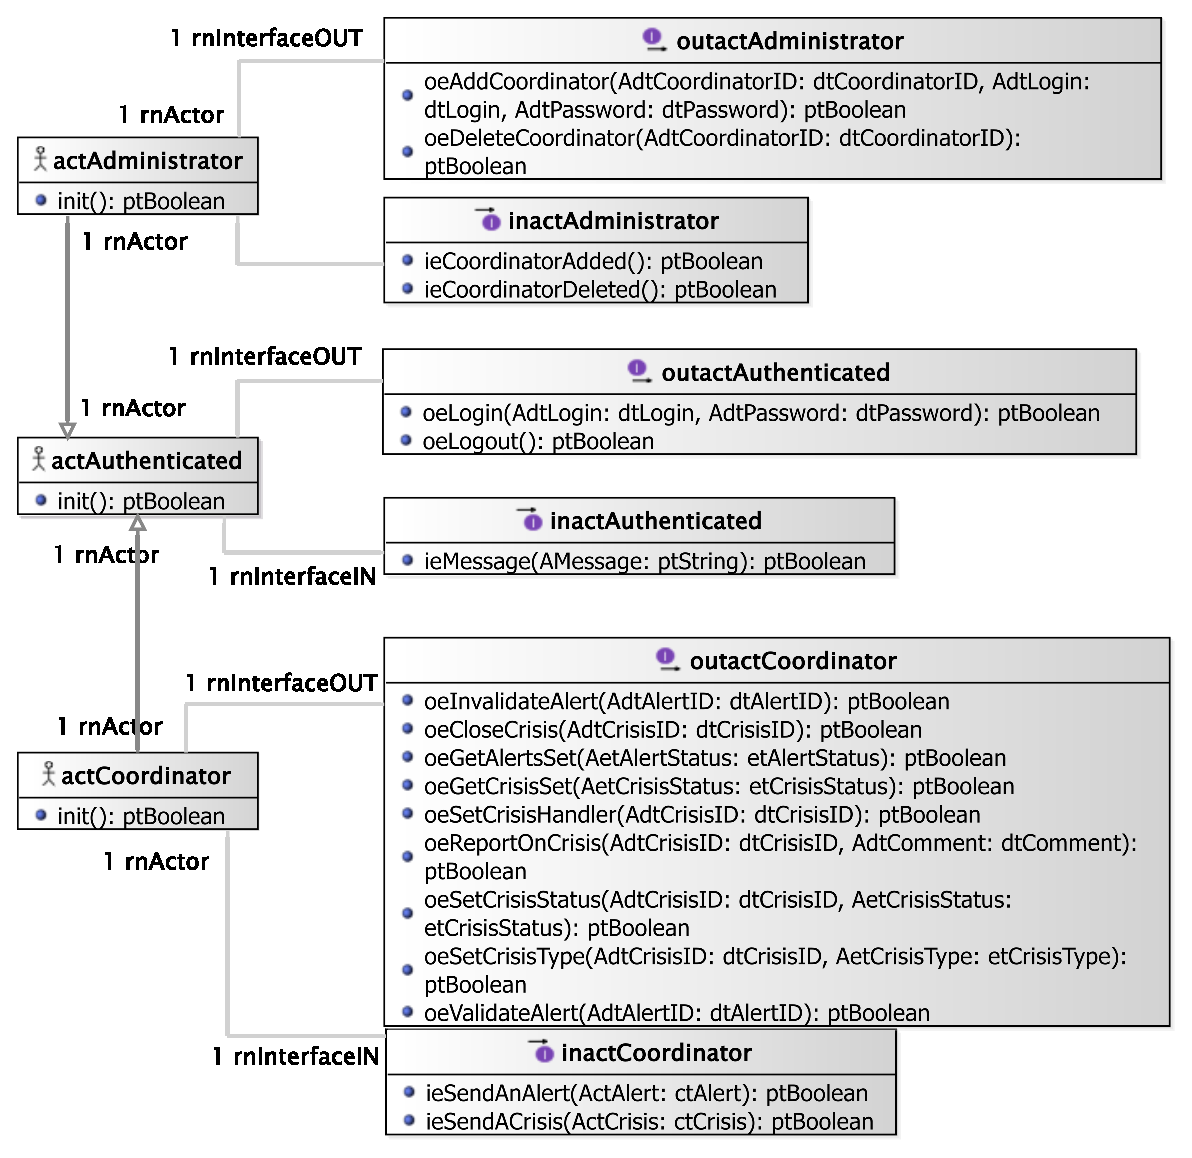
\includegraphics[
angle=0
,scale=0.80
]{./images-report-gen/environment-model/local/01/em-lv-01.eps}
\end{center}
\caption[Environment Model - Local View 01 - environment model local view - Part ]{Environment Model - Local View 01. environment model local view - Part 1.}
\label{fig:lu.uni.lassy.excalibur.examples.icrash-EM-view-local-01}
\end{figure}
\vspace{0.5cm} 

\section{Local view 02}
\label{sec:lu.uni.lassy.excalibur.examples.icrash-EM-view-02-local}

Figure \ref{fig:lu.uni.lassy.excalibur.examples.icrash-EM-view-local-02} 
shows the local view giving the second part the environment model of the system in term of its state class, actors with their input and output interfaces and all related associations.


\begin{figure}[htbp] 
\label{fig:lu.uni.lassy.excalibur.examples.icrash-EM}
\begin{center}
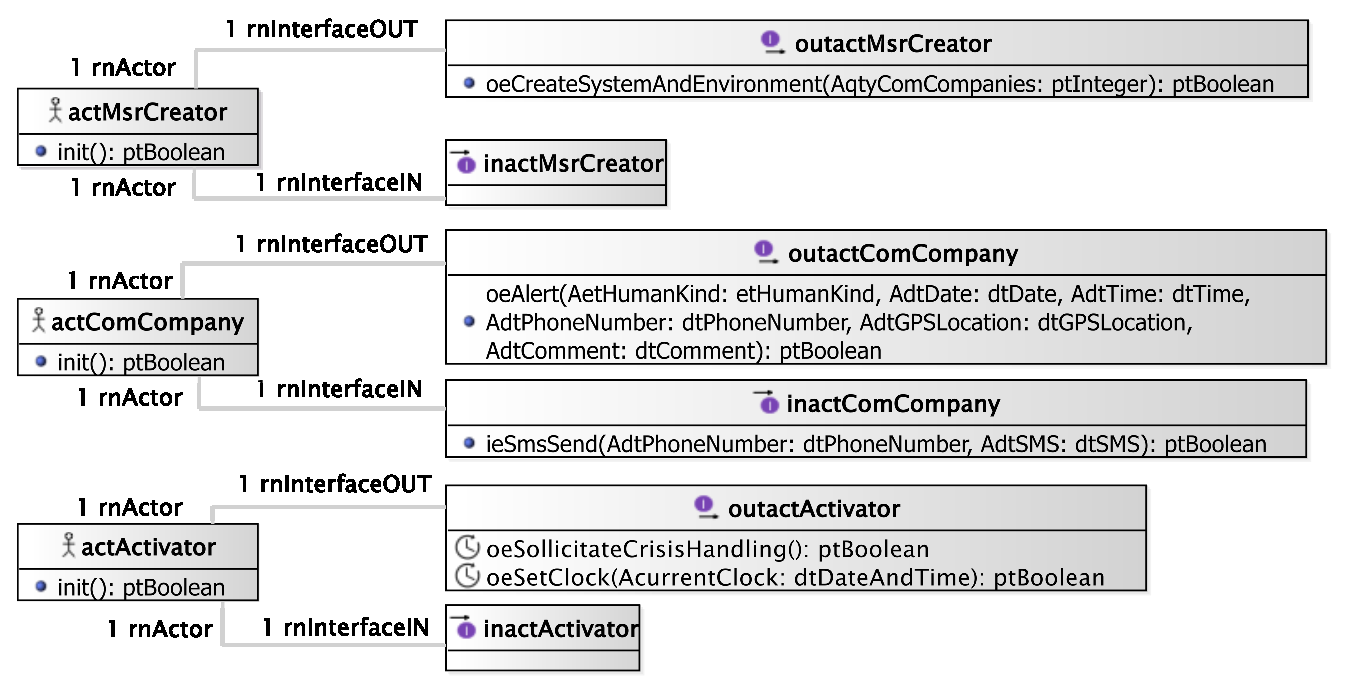
\includegraphics[
angle=0
,scale=0.80
]{./images-report-gen/environment-model/local/02/em-lv-02.eps}
\end{center}
\caption[Environment Model - Local View 02 - environment model local view - Part ]{Environment Model - Local View 02. environment model local view - Part 2.}
\label{fig:lu.uni.lassy.excalibur.examples.icrash-EM-view-local-02}
\end{figure}
\vspace{0.5cm} 

\section{Local view 03}
\label{sec:lu.uni.lassy.excalibur.examples.icrash-EM-view-03-local}

Figure \ref{fig:lu.uni.lassy.excalibur.examples.icrash-EM-view-local-03} shows the local view for the administrator actor and interfaces


\begin{figure}[htbp] 
\label{fig:lu.uni.lassy.excalibur.examples.icrash-EM}
\begin{center}
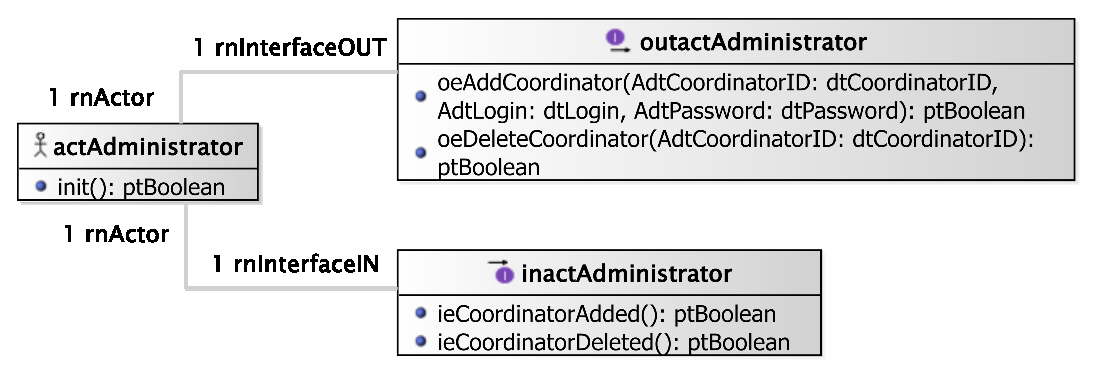
\includegraphics[
angle=0
,scale=0.80
]{./images-report-gen/environment-model/local/03/em-lv-03-parta-administrator.eps}
\end{center}
\caption[Environment Model - Local View 03 - administrator actor environment mode]{Environment Model - Local View 03. administrator actor environment model view.}
\label{fig:lu.uni.lassy.excalibur.examples.icrash-EM-view-local-03}
\end{figure}
\vspace{0.5cm} 

\section{Local view 04}
\label{sec:lu.uni.lassy.excalibur.examples.icrash-EM-view-04-local}

Figure \ref{fig:lu.uni.lassy.excalibur.examples.icrash-EM-view-local-04} shows the local view for the coordinator actor and interfaces


\begin{figure}[htbp] 
\label{fig:lu.uni.lassy.excalibur.examples.icrash-EM}
\begin{center}
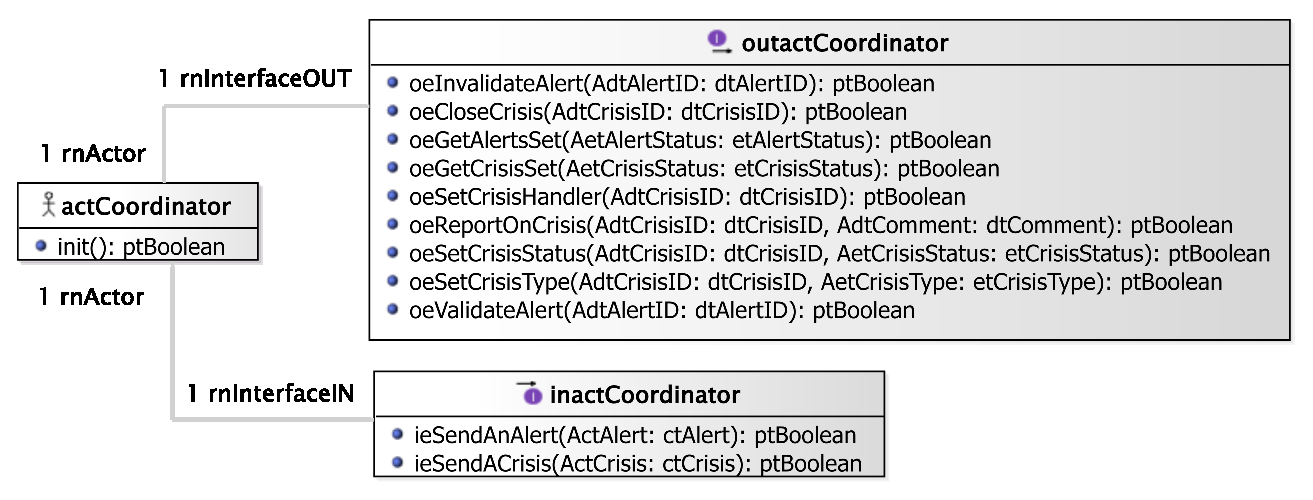
\includegraphics[
angle=0
,scale=0.80
]{./images-report-gen/environment-model/local/04/em-lv-04-partb-coordinator.eps}
\end{center}
\caption[Environment Model - Local View 04 - coordinator actor environment model ]{Environment Model - Local View 04. coordinator actor environment model view.}
\label{fig:lu.uni.lassy.excalibur.examples.icrash-EM-view-local-04}
\end{figure}
\vspace{0.5cm} 

\section{Local view 05}
\label{sec:lu.uni.lassy.excalibur.examples.icrash-EM-view-05-local}

Figure \ref{fig:lu.uni.lassy.excalibur.examples.icrash-EM-view-local-05} shows the local view for the authenticated actor and interfaces


\begin{figure}[htbp] 
\label{fig:lu.uni.lassy.excalibur.examples.icrash-EM}
\begin{center}
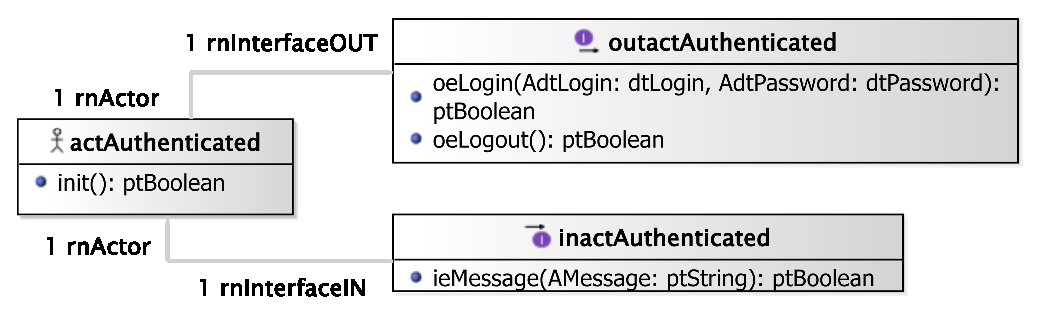
\includegraphics[
angle=0
,scale=0.80
]{./images-report-gen/environment-model/local/05/em-lv-05-partc-authenticated.eps}
\end{center}
\caption[Environment Model - Local View 05 - authenticated actor environment mode]{Environment Model - Local View 05. authenticated actor environment model local view.}
\label{fig:lu.uni.lassy.excalibur.examples.icrash-EM-view-local-05}
\end{figure}
\vspace{0.5cm} 



\section{Global view 01}
\label{sec:lu.uni.lassy.excalibur.examples.icrash-EM-view-01-global}
\clearpage

Figure \ref{fig:lu.uni.lassy.excalibur.examples.icrash-EM-view-global-01} shows a global view for all actors with their relationships with ctState


\begin{figure}[htbp] 
\label{fig:lu.uni.lassy.excalibur.examples.icrash-EM}
\begin{center}
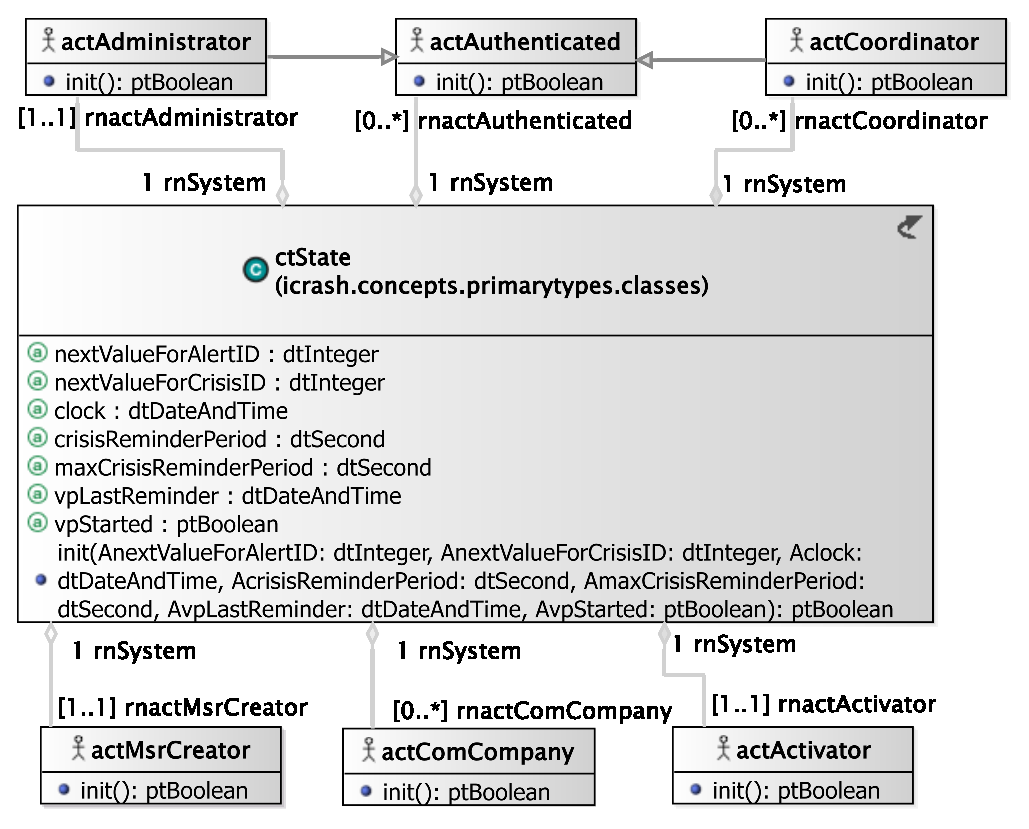
\includegraphics[
angle=0
,scale=0.80
]{./images-report-gen/environment-model/global/01/em-gv-01.eps}
\end{center}
\caption[Environment Model - Global View 01 -  em-gv-01 environment model global v]{Environment Model - Global View 01.  em-gv-01 environment model global view.}
\label{fig:lu.uni.lassy.excalibur.examples.icrash-EM-view-global-01}
\end{figure}
\vspace{0.5cm} 




\section{Actors and Interfaces Descriptions}
\label{sec:lu.uni.lassy.excalibur.examples.icrash-EM-Actors-Descriptions}


		
We provide for the given views the description of the actors together with their associated input and output interface descriptions.
\subsection{\msrcode{actActivator} Actor}


\begin{actortable}
	\addheading{Actor}
	
	\adddoublerow{actActivator}{represents a logical actor for time automatic message sending based on system's or environment status.}
	
	
	
	
	

	\addrowheading{OutputInterfaces}
	\addnumbereddoublerow{OUT}{\hypertarget{actActivator.outactActivator.oeSollicitateCrisisHandling}
			{\msrcode{[proactive] oeSollicitateCrisisHandling():ptBoolean}}}
			{used to avoid crisis to stay too long in an not handled status.}
	\addnumbereddoublerow{OUT}{\hypertarget{actActivator.outactActivator.oeSetClock}
			{\msrcode{[proactive] oeSetClock(AcurrentClock:dtDateAndTime):ptBoolean}}}
			{used to update the system's time}
	
	
\end{actortable}

\subsection{\msrcode{actAdministrator} Actor}


\begin{actortable}
	\addheading{Actor}
	
	\adddoublerow{actAdministrator}{represents an actor responsible of administration tasks for the \msricrash system.}
	
	\addrowheading{Extends}
	\addsinglerow{icrash.environment.actAuthenticated}
	
	
	
	
	

	\addrowheading{OutputInterfaces}
	\addnumbereddoublerow{OUT}{\hypertarget{actAdministrator.outactAdministrator.oeAddCoordinator}
			{\msrcode{oeAddCoordinator(AdtCoordinatorID:dtCoordinatorID, AdtLogin:dtLogin, AdtPassword:dtPassword):ptBoolean}}}
			{sent to add a new coordinator in the system's post state and environment's post state.}
	\addnumbereddoublerow{OUT}{\hypertarget{actAdministrator.outactAdministrator.oeDeleteCoordinator}
			{\msrcode{oeDeleteCoordinator(AdtCoordinatorID:dtCoordinatorID):ptBoolean}}}
			{sent to delete an existing coordinator in the system's post state and environment's post state.}
	
	\addrowheading{InputInterfaces}
	\addnumbereddoublerow{IN}{\msrcode{ieCoordinatorAdded():ptBoolean}}
							 {its reception confirms the creation of the requested coodinator. }
	\addnumbereddoublerow{IN}{\msrcode{ieCoordinatorDeleted():ptBoolean}}
							 {its reception confirms the deletion of the requested coodinator. }
	
\end{actortable}

\subsection{\msrcode{actAuthenticated} Actor}


\begin{actortable}
	\addheading{Actor}
	
	\adddoublerow{actAuthenticated}{abstract actor providing reusable input and output interfaces for actors that need to authenticate themselves.}
	
	
	
	
	

	\addrowheading{OutputInterfaces}
	\addnumbereddoublerow{OUT}{\hypertarget{actAuthenticated.outactAuthenticated.oeLogin}
			{\msrcode{oeLogin(AdtLogin:dtLogin, AdtPassword:dtPassword):ptBoolean}}}
			{sent to request authorization to request access secured system operations.}
	\addnumbereddoublerow{OUT}{\hypertarget{actAuthenticated.outactAuthenticated.oeLogout}
			{\msrcode{oeLogout():ptBoolean}}}
			{sent to end the secured access to specific system operations.}
	
	\addrowheading{InputInterfaces}
	\addnumbereddoublerow{IN}{\msrcode{ieMessage(AMessage:ptString):ptBoolean}}
							 {allows for receiving general textual messages.}
	
\end{actortable}

\subsection{\msrcode{actComCompany} Actor}


\begin{actortable}
	\addheading{Actor}
	
	\adddoublerow{actComCompany}{represents the communication company stakeholder ensuring the input/ouput of textual messages with humans having communicaiton devices.}
	
	
	
	
	

	\addrowheading{OutputInterfaces}
	\addnumbereddoublerow{OUT}{\hypertarget{actComCompany.outactComCompany.oeAlert}
			{\msrcode{oeAlert(AetHumanKind:etHumanKind, AdtDate:dtDate, AdtTime:dtTime, AdtPhoneNumber:dtPhoneNumber, AdtGPSLocation:dtGPSLocation, AdtComment:dtComment):ptBoolean}}}
			{sent to alert of a potential crisis situation.}
	
	\addrowheading{InputInterfaces}
	\addnumbereddoublerow{IN}{\msrcode{ieSmsSend(AdtPhoneNumber:dtPhoneNumber, AdtSMS:dtSMS):ptBoolean}}
							 {allows for receiving textual messages to be dispatched to the communication company customers having the provided phone number.}
	
\end{actortable}

\subsection{\msrcode{actCoordinator} Actor}


\begin{actortable}
	\addheading{Actor}
	
	\adddoublerow{actCoordinator}{represents actor responsible of handling one or several crisis for the \msricrash system.}
	
	\addrowheading{Extends}
	\addsinglerow{icrash.environment.actAuthenticated}
	
	
	
	
	

	\addrowheading{OutputInterfaces}
	\addnumbereddoublerow{OUT}{\hypertarget{actCoordinator.outactCoordinator.oeInvalidateAlert}
			{\msrcode{oeInvalidateAlert(AdtAlertID:dtAlertID):ptBoolean}}}
			{sent to indicate that an alert should be considered as closed.}
	\addnumbereddoublerow{OUT}{\hypertarget{actCoordinator.outactCoordinator.oeCloseCrisis}
			{\msrcode{oeCloseCrisis(AdtCrisisID:dtCrisisID):ptBoolean}}}
			{sent to indicate that a crisis should be considered as closed.}
	\addnumbereddoublerow{OUT}{\hypertarget{actCoordinator.outactCoordinator.oeGetAlertsSet}
			{\msrcode{oeGetAlertsSet(AetAlertStatus:etAlertStatus):ptBoolean}}}
			{sent to request all the ctAlert instances having a specific status.}
	\addnumbereddoublerow{OUT}{\hypertarget{actCoordinator.outactCoordinator.oeGetCrisisSet}
			{\msrcode{oeGetCrisisSet(AetCrisisStatus:etCrisisStatus):ptBoolean}}}
			{sent to request all the ctCrisis instances having a specific status.}
	\addnumbereddoublerow{OUT}{\hypertarget{actCoordinator.outactCoordinator.oeSetCrisisHandler}
			{\msrcode{oeSetCrisisHandler(AdtCrisisID:dtCrisisID):ptBoolean}}}
			{sent to declare himself as been the handler of a crisis having the specified id.}
	\addnumbereddoublerow{OUT}{\hypertarget{actCoordinator.outactCoordinator.oeReportOnCrisis}
			{\msrcode{oeReportOnCrisis(AdtCrisisID:dtCrisisID, AdtComment:dtComment):ptBoolean}}}
			{sent to update the textual information available for a specific handled crisis.}
	\addnumbereddoublerow{OUT}{\hypertarget{actCoordinator.outactCoordinator.oeSetCrisisStatus}
			{\msrcode{oeSetCrisisStatus(AdtCrisisID:dtCrisisID, AetCrisisStatus:etCrisisStatus):ptBoolean}}}
			{sent to define the handling status of a specific crisis.}
	\addnumbereddoublerow{OUT}{\hypertarget{actCoordinator.outactCoordinator.oeSetCrisisType}
			{\msrcode{oeSetCrisisType(AdtCrisisID:dtCrisisID, AetCrisisType:etCrisisType):ptBoolean}}}
			{sent to define the gravity type of a specific crisis.}
	\addnumbereddoublerow{OUT}{\hypertarget{actCoordinator.outactCoordinator.oeValidateAlert}
			{\msrcode{oeValidateAlert(AdtAlertID:dtAlertID):ptBoolean}}}
			{sent to indicate that a specific alert is not a fake.}
	
	\addrowheading{InputInterfaces}
	\addnumbereddoublerow{IN}{\msrcode{ieSendAnAlert(ActAlert:ctAlert):ptBoolean}}
							 {allows for receiving a requested ctAlert instance.}
	\addnumbereddoublerow{IN}{\msrcode{ieSendACrisis(ActCrisis:ctCrisis):ptBoolean}}
							 {allows for receiving a requested ctCrisis instance.}
	
\end{actortable}

\subsection{\msrcode{actMsrCreator} Actor}


\begin{actortable}
	\addheading{Actor}
	
	\adddoublerow{actMsrCreator}{Represents the creator stakeholder in charge of state and environment initialization.}
	
	
	
	
	

	\addrowheading{OutputInterfaces}
	\addnumbereddoublerow{OUT}{\hypertarget{actMsrCreator.outactMsrCreator.oeCreateSystemAndEnvironment}
			{\msrcode{oeCreateSystemAndEnvironment(AqtyComCompanies:ptInteger):ptBoolean}}}
			{sent to request the initialization of the system's class instances and the environment actors instances.}
	
	
\end{actortable}




\chapter{Concept Model}
\label{chap:lu.uni.lassy.excalibur.examples.icrash-CM}


\section{PrimaryTypes-Classes}
\subsection{Local view 01}
\label{sec:lu.uni.lassy.excalibur.examples.icrash-CM-view-local-PrimaryTypes-Classes-01}
Figure \ref{fig:lu.uni.lassy.excalibur.examples.icrash-CM-view-local-PrimaryTypes-Classes-01} 
shows the local view on all the primary types class types.



\begin{figure}[htbp] 
\label{fig:lu.uni.lassy.excalibur.examples.icrash-CM}
\begin{center}
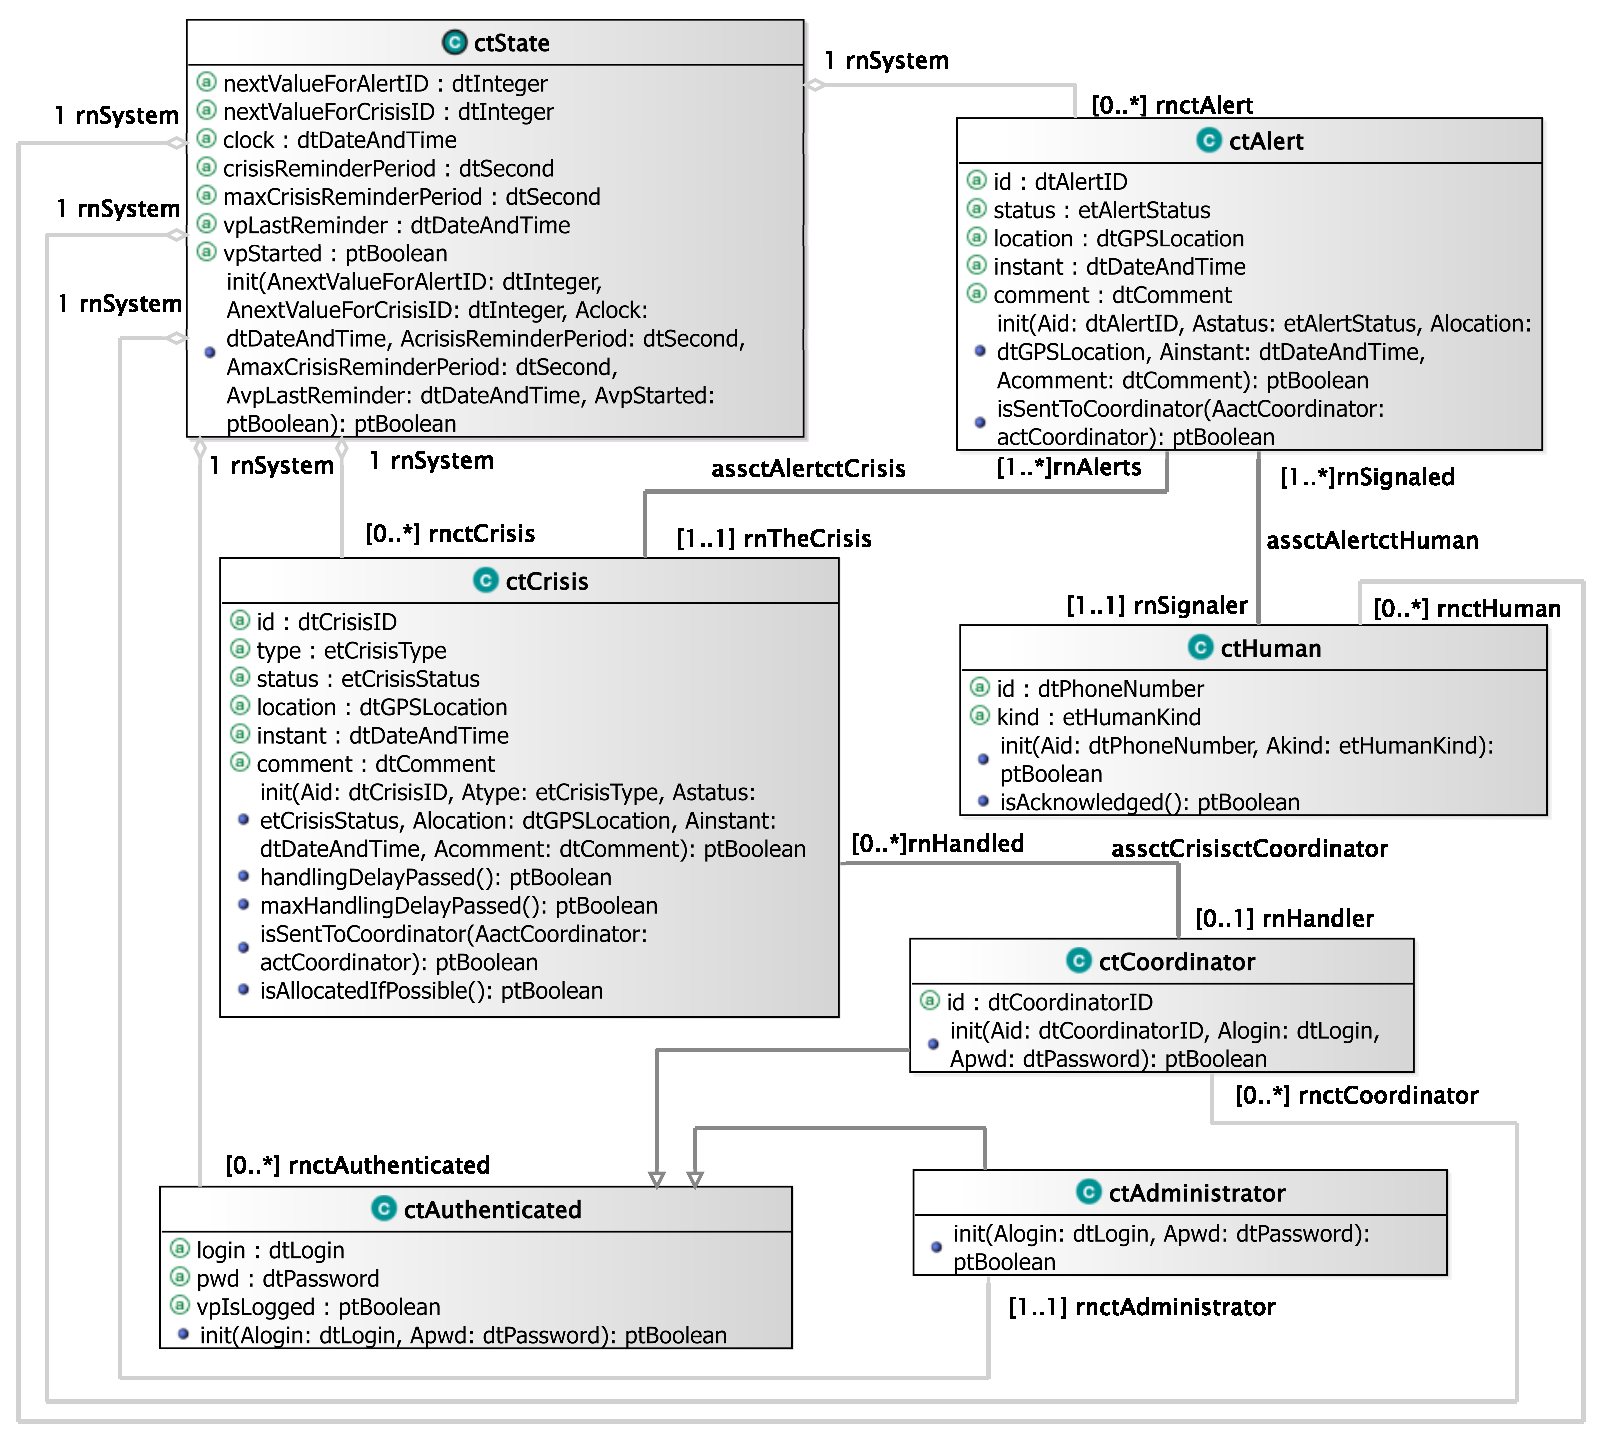
\includegraphics[
angle=0
,width=1.0\textwidth
]{./images-report-gen/concept-model/local/PrimaryTypes-Classes/01/cm-pt-ct-lv-01.eps}
\end{center}
\caption[Concept Model - PrimaryTypes-Classes local view 01 - Local view of all the primary types ]{Concept Model - PrimaryTypes-Classes local view 01. Local view of all the primary types class types
.}
\label{fig:lu.uni.lassy.excalibur.examples.icrash-CM-view-local-PrimaryTypes-Classes-01}
\end{figure}
\vspace{0.5cm} 

\subsection{Local view 02}
\label{sec:lu.uni.lassy.excalibur.examples.icrash-CM-view-local-PrimaryTypes-Classes-02}
Figure \ref{fig:lu.uni.lassy.excalibur.examples.icrash-CM-view-local-PrimaryTypes-Classes-02} shows the local view of the ctState primary type class type.



\begin{figure}[htbp] 
\label{fig:lu.uni.lassy.excalibur.examples.icrash-CM}
\begin{center}
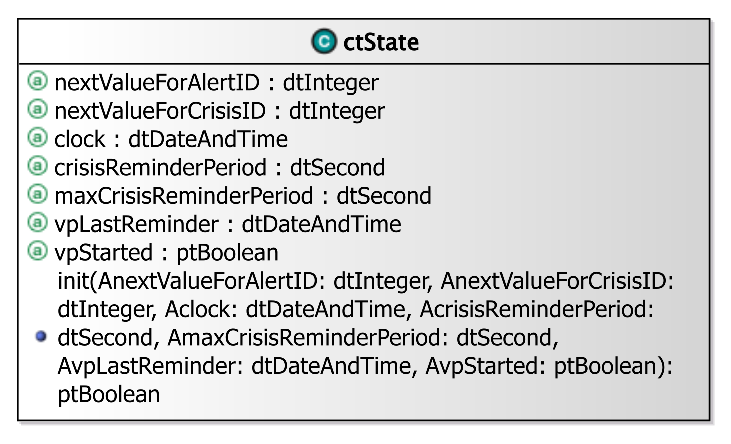
\includegraphics[
angle=0
,scale=0.80
]{./images-report-gen/concept-model/local/PrimaryTypes-Classes/02/cm-pt-ct-lv-02-parta-ctState.eps}
\end{center}
\caption[Concept Model - PrimaryTypes-Classes local view 02 - local view of the ctState primary ty]{Concept Model - PrimaryTypes-Classes local view 02. local view of the ctState primary type.}
\label{fig:lu.uni.lassy.excalibur.examples.icrash-CM-view-local-PrimaryTypes-Classes-02}
\end{figure}
\vspace{0.5cm} 

\subsection{Local view 03}
\label{sec:lu.uni.lassy.excalibur.examples.icrash-CM-view-local-PrimaryTypes-Classes-03}
Figure \ref{fig:lu.uni.lassy.excalibur.examples.icrash-CM-view-local-PrimaryTypes-Classes-03} shows the local view of the ctAlert primary type class type.



\begin{figure}[htbp] 
\label{fig:lu.uni.lassy.excalibur.examples.icrash-CM}
\begin{center}
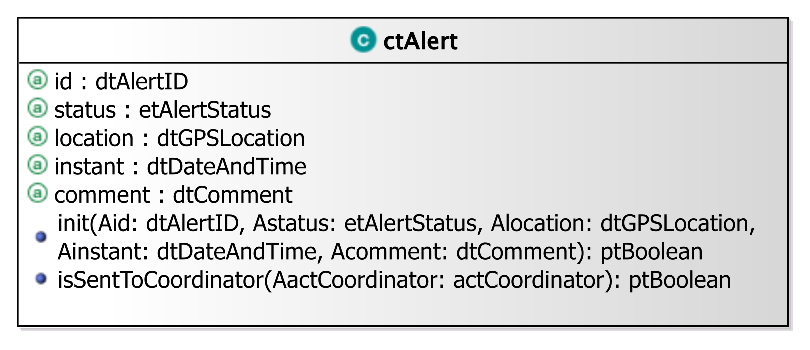
\includegraphics[
angle=0
,scale=0.80
]{./images-report-gen/concept-model/local/PrimaryTypes-Classes/03/cm-pt-ct-lv-03-partb-ctAlert.eps}
\end{center}
\caption[Concept Model - PrimaryTypes-Classes local view 03 - local view of the ctAlert primary ty]{Concept Model - PrimaryTypes-Classes local view 03. local view of the ctAlert primary type.}
\label{fig:lu.uni.lassy.excalibur.examples.icrash-CM-view-local-PrimaryTypes-Classes-03}
\end{figure}
\vspace{0.5cm} 

\subsection{Local view 04}
\label{sec:lu.uni.lassy.excalibur.examples.icrash-CM-view-local-PrimaryTypes-Classes-04}
Figure \ref{fig:lu.uni.lassy.excalibur.examples.icrash-CM-view-local-PrimaryTypes-Classes-04} shows the local view of the ctCrisis primary type class type.



\begin{figure}[htbp] 
\label{fig:lu.uni.lassy.excalibur.examples.icrash-CM}
\begin{center}
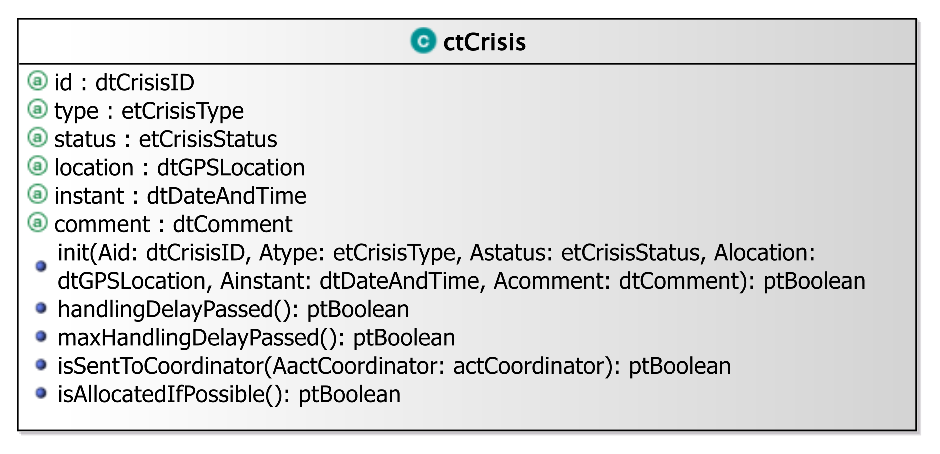
\includegraphics[
angle=0
,scale=0.80
]{./images-report-gen/concept-model/local/PrimaryTypes-Classes/04/cm-pt-ct-lv-04-partc-ctCrisis.eps}
\end{center}
\caption[Concept Model - PrimaryTypes-Classes local view 04 - local view of the ctCrisis primary t]{Concept Model - PrimaryTypes-Classes local view 04. local view of the ctCrisis primary type.}
\label{fig:lu.uni.lassy.excalibur.examples.icrash-CM-view-local-PrimaryTypes-Classes-04}
\end{figure}
\vspace{0.5cm} 


\subsection{Global view 01}
\label{sec:lu.uni.lassy.excalibur.examples.icrash-CM-view-global-PrimaryTypes-Classes-01}
Figure \ref{fig:lu.uni.lassy.excalibur.examples.icrash-CM-view-global-PrimaryTypes-Classes-01} 
shows the global view on primary types class types showing the association(s) types with the actor classes of the environment model.



\begin{figure}[htbp] 
\label{fig:lu.uni.lassy.excalibur.examples.icrash-CM}
\begin{center}
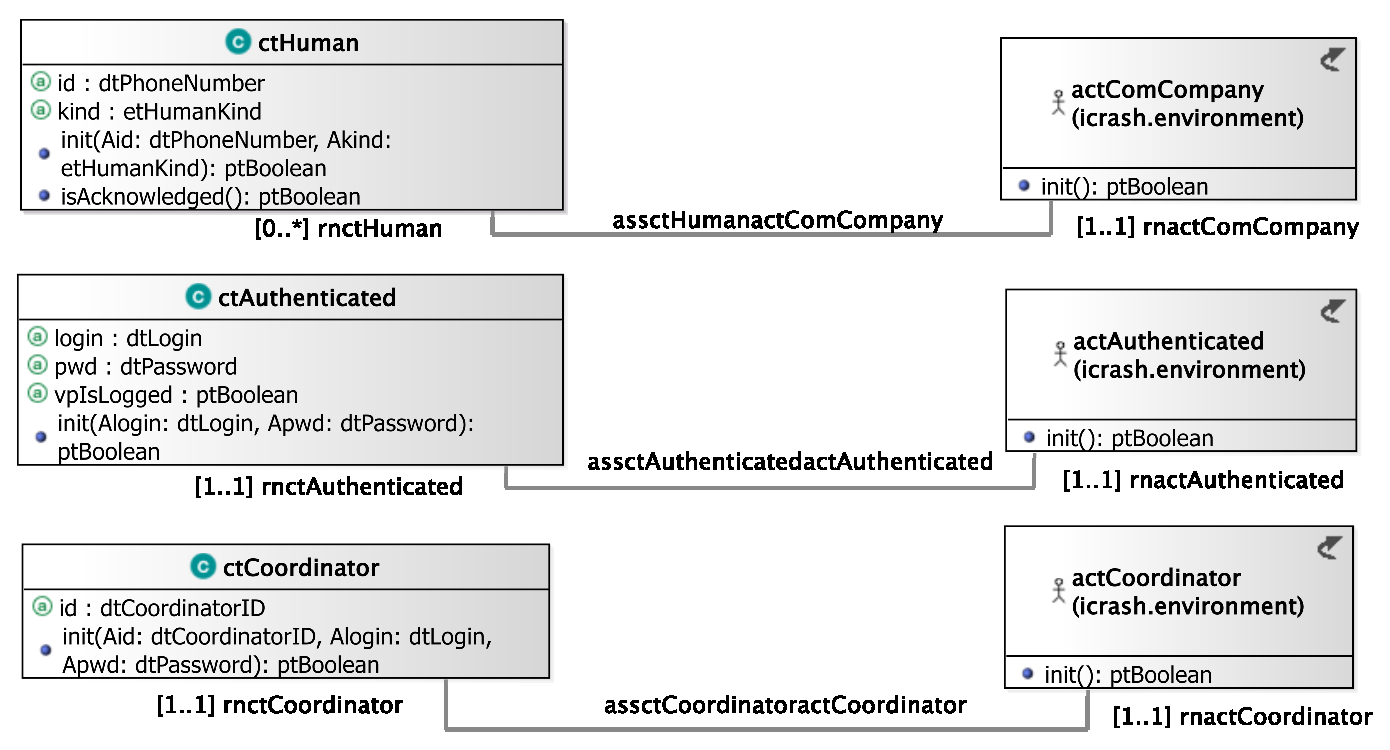
\includegraphics[
angle=0
,width=1.0\textwidth
]{./images-report-gen/concept-model/global/PrimaryTypes-Classes/01/cm-pt-ct-gv-01.eps}
\end{center}
\caption[Concept Model - PrimaryTypes-Classes global view 01 -  Primary types class types global vi]{Concept Model - PrimaryTypes-Classes global view 01.  Primary types class types global view - cm-pt-ct-gv-01
.}
\label{fig:lu.uni.lassy.excalibur.examples.icrash-CM-view-global-PrimaryTypes-Classes-01}
\end{figure}
\vspace{0.5cm} 



\section{PrimaryTypes-Datatypes}
\subsection{Local view 06}
\label{sec:lu.uni.lassy.excalibur.examples.icrash-CM-view-local-PrimaryTypes-Datatypes-06}
Figure \ref{fig:lu.uni.lassy.excalibur.examples.icrash-CM-view-local-PrimaryTypes-Datatypes-06} 



\begin{figure}[htbp] 
\label{fig:lu.uni.lassy.excalibur.examples.icrash-CM}
\begin{center}
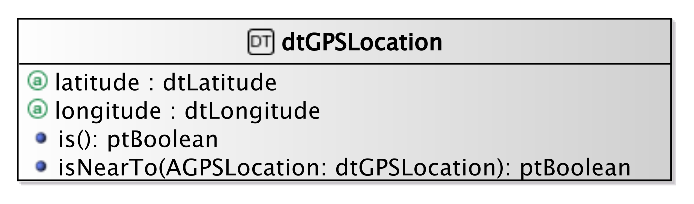
\includegraphics[
angle=0
]{./images-report-gen/concept-model/local/PrimaryTypes-Datatypes/06/cm-pt-dt-lv-02-dtGPSLocation.eps}
\end{center}
\caption[Concept Model - PrimaryTypes-Datatypes local view 06 - ]{Concept Model - PrimaryTypes-Datatypes local view 06. .}
\label{fig:lu.uni.lassy.excalibur.examples.icrash-CM-view-local-PrimaryTypes-Datatypes-06}
\end{figure}
\vspace{0.5cm} 


\subsection{Global view 01}
\label{sec:lu.uni.lassy.excalibur.examples.icrash-CM-view-global-PrimaryTypes-Datatypes-01}
Figure \ref{fig:lu.uni.lassy.excalibur.examples.icrash-CM-view-global-PrimaryTypes-Datatypes-01} 
shows a global view on the \msricrash primary types datatype types.



\begin{figure}[htbp] 
\label{fig:lu.uni.lassy.excalibur.examples.icrash-CM}
\begin{center}
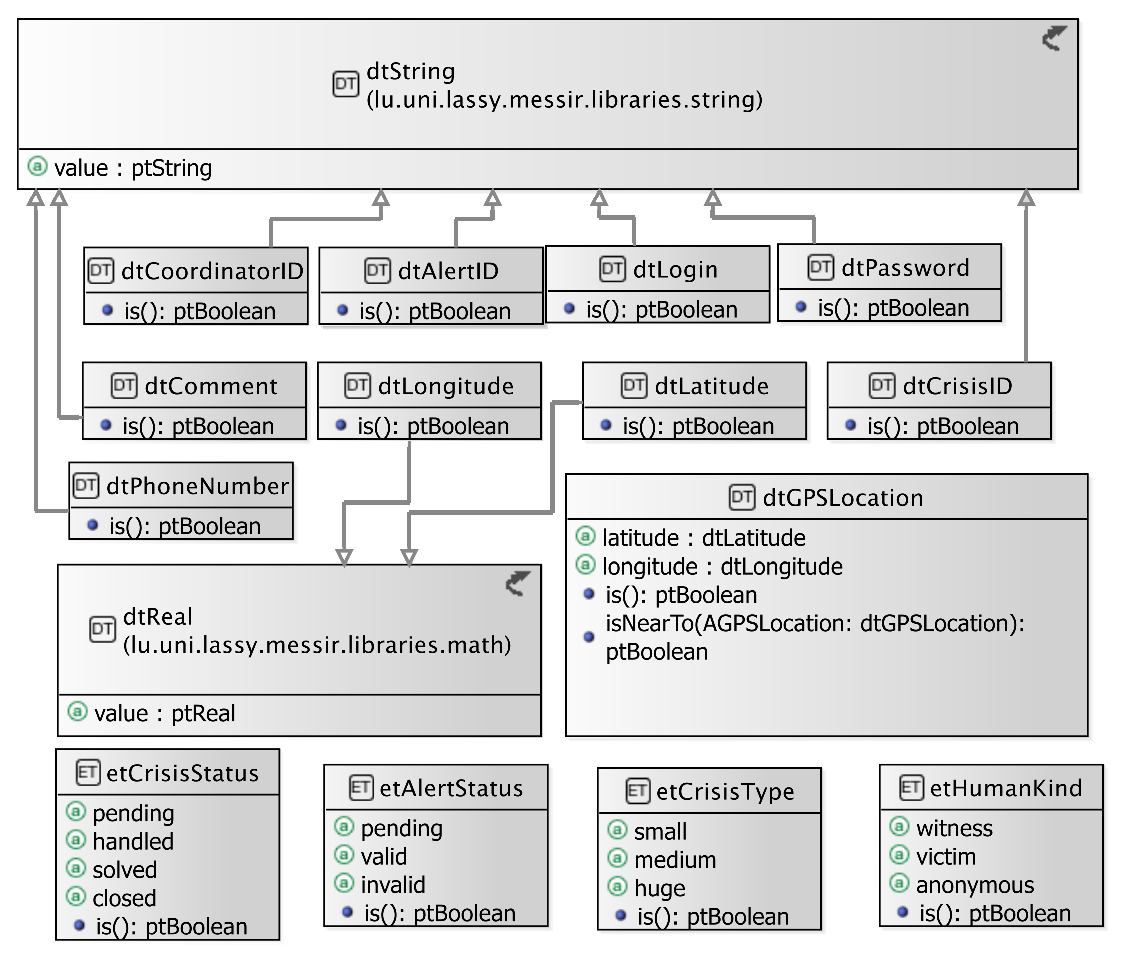
\includegraphics[
angle=0
,width=1.0\textwidth
]{./images-report-gen/concept-model/global/PrimaryTypes-Datatypes/01/cm-pt-dt-gv-01.eps}
\end{center}
\caption[Concept Model - PrimaryTypes-Datatypes global view 01 -  global view of primary types dataty]{Concept Model - PrimaryTypes-Datatypes global view 01.  global view of primary types datatype types - cm-pt-dt-gv-01
.}
\label{fig:lu.uni.lassy.excalibur.examples.icrash-CM-view-global-PrimaryTypes-Datatypes-01}
\end{figure}
\vspace{0.5cm} 





\section{SecondaryTypes-Datatypes}
\subsection{Local view 01}
\label{sec:lu.uni.lassy.excalibur.examples.icrash-CM-view-local-SecondaryTypes-Datatypes-01}
Figure \ref{fig:lu.uni.lassy.excalibur.examples.icrash-CM-view-local-SecondaryTypes-Datatypes-01} shows the local view of the secondary types datatype types.



\begin{figure}[htbp] 
\label{fig:lu.uni.lassy.excalibur.examples.icrash-CM}
\begin{center}
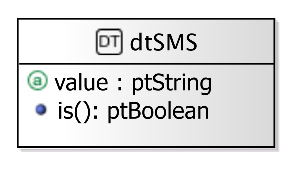
\includegraphics[
angle=0
]{./images-report-gen/concept-model/local/SecondaryTypes-Datatypes/01/cm-st-dt-lv-01.eps}
\end{center}
\caption[Concept Model - SecondaryTypes-Datatypes local view 01 - Local view of the secondary types da]{Concept Model - SecondaryTypes-Datatypes local view 01. Local view of the secondary types datatype types.}
\label{fig:lu.uni.lassy.excalibur.examples.icrash-CM-view-local-SecondaryTypes-Datatypes-01}
\end{figure}
\vspace{0.5cm} 






\section{Concept Model Types Descriptions}
This section provides the textual descriptions of all the types defined in the concept model and that can be part of the graphical views provided.

\subsection{Primary types - Class types descriptions}




The table below is providing comments on the graphical views given for the class types of the primary types. Type logical operations are precisely specified in the operation model.

\begin{datadictionary}
\addheading{Classes}

\adddoublerow{ctAdministrator}{used to caracterize internally the entity that is responsible of administrating the \msricrash system.}
\addsingletwocolumnrow{extends}{icrash.concepts.primarytypes.classes.ctAuthenticated}
\adddoubletwocolumnrow{operation}{\msrcode{init(Alogin:dtLogin, Apwd:dtPassword):ptBoolean}}{used to initialize the current object as a new instance of the ctAdministrator type.}
\adddoublerow{ctAlert}{Used to model crisis alerts sent by any human having communication capability using communication companies belonging to the system's environment}
\adddoubletwocolumnrow{attribute}{\msrcode{comment: dtComment}}{a textual description providing unstructured information on the alert.}
\adddoubletwocolumnrow{attribute}{\msrcode{id: dtAlertID}}{the alert unique identification information.}
\adddoubletwocolumnrow{attribute}{\msrcode{instant: dtDateAndTime}}{the date and time at which the alert notification has been sent.}
\adddoubletwocolumnrow{attribute}{\msrcode{location: dtGPSLocation}}{the position of the alert provided by the space-based satellite navigation system used by the human using the communication company to inform the \msricrash system of a crisis.}
\adddoubletwocolumnrow{attribute}{\msrcode{status: etAlertStatus}}{the alert validation status }
\adddoubletwocolumnrow{operation}{\msrcode{init(Aid:dtAlertID, Astatus:etAlertStatus, Alocation:dtGPSLocation, Ainstant:dtDateAndTime, Acomment:dtComment):ptBoolean}}{used to initialize the current object as a new instance of the ctAlert type.}
\adddoubletwocolumnrow{operation}{\msrcode{isSentToCoordinator(AactCoordinator:actCoordinator):ptBoolean}}{used to provide a given coordinator with current alert information.}
\adddoublerow{ctAuthenticated}{used to model system's representation about actors that need to authenticate to access some specific functionalities.}
\adddoubletwocolumnrow{attribute}{\msrcode{login: dtLogin}}{an identifier for authentication.}
\adddoubletwocolumnrow{attribute}{\msrcode{pwd: dtPassword}}{a key for authentication.}
\adddoubletwocolumnrow{attribute}{\msrcode{vpIsLogged: ptBoolean}}{used to determine the access status.}
\adddoubletwocolumnrow{operation}{\msrcode{init(Alogin:dtLogin, Apwd:dtPassword):ptBoolean}}{used to initialize the current object as a new instance of the ctAuthenticated type.}
\adddoublerow{ctCoordinator}{used to model system's representation about the actors that have the responsibility to handle alerts and crisis.}
\addsingletwocolumnrow{extends}{icrash.concepts.primarytypes.classes.ctAuthenticated}
\adddoubletwocolumnrow{attribute}{\msrcode{id: dtCoordinatorID}}{a unique identification information.}
\adddoubletwocolumnrow{operation}{\msrcode{init(Aid:dtCoordinatorID, Alogin:dtLogin, Apwd:dtPassword):ptBoolean}}{used to initialize the current object as a new instance of the ctCoordinator type.}
\adddoublerow{ctCrisis}{Used to model crisis that are infered from the reception of at least one alert message. Crisis aer entities that are handled by the \msricrash system.}
\adddoubletwocolumnrow{attribute}{\msrcode{comment: dtComment}}{a textual description providing unstructured information on the crisis handling.}
\adddoubletwocolumnrow{attribute}{\msrcode{id: dtCrisisID}}{the crisis unique identification information.}
\adddoubletwocolumnrow{attribute}{\msrcode{instant: dtDateAndTime}}{the date and time at which the first related alert notification has been sent.}
\adddoubletwocolumnrow{attribute}{\msrcode{location: dtGPSLocation}}{the position of the crisis equal by the one of the first alert received and associated to the crisis.}
\adddoubletwocolumnrow{attribute}{\msrcode{status: etCrisisStatus}}{the crisis handling status.}
\adddoubletwocolumnrow{attribute}{\msrcode{type: etCrisisType}}{an indication of the gravity of the crisis.}
\adddoubletwocolumnrow{operation}{\msrcode{handlingDelayPassed():ptBoolean}}{used to determine if the crisis stood too longly in a pending status since last reminder.}
\adddoubletwocolumnrow{operation}{\msrcode{init(Aid:dtCrisisID, Atype:etCrisisType, Astatus:etCrisisStatus, Alocation:dtGPSLocation, Ainstant:dtDateAndTime, Acomment:dtComment):ptBoolean}}{used to initialize the current object as a new instance of the ctAlert type.}
\adddoubletwocolumnrow{operation}{\msrcode{isAllocatedIfPossible():ptBoolean}}{used to allocate a crisis to a coordinator if any or to alert the administrator of crisis waiting to be handled.}
\adddoubletwocolumnrow{operation}{\msrcode{isSentToCoordinator(AactCoordinator:actCoordinator):ptBoolean}}{used to provide a given coordinator with current crisis information.}
\adddoubletwocolumnrow{operation}{\msrcode{maxHandlingDelayPassed():ptBoolean}}{used to determine if the crisis stood too longly in a pending status since its creation.}
\adddoublerow{ctHuman}{used to model system's representation about the indirect actors that has alerted of potential crisis.}
\adddoubletwocolumnrow{attribute}{\msrcode{id: dtPhoneNumber}}{the number of the communication device used to send an alert to \msricrash system.}
\adddoubletwocolumnrow{attribute}{\msrcode{kind: etHumanKind}}{role with respect to the alert notified.}
\adddoubletwocolumnrow{operation}{\msrcode{init(Aid:dtPhoneNumber, Akind:etHumanKind):ptBoolean}}{\msrcode{init}: used to initialize the current object as a new instance of the ctHuman type.}
\adddoublerow{ctState}{used to model the system. Each system specified using \msrmessir must include a ctState class for which there is only one instance at any state of the abstract machine after creation.}
\adddoubletwocolumnrow{attribute}{\msrcode{clock: dtDateAndTime}}{used to represent the system local time.}
\adddoubletwocolumnrow{attribute}{\msrcode{crisisReminderPeriod: dtSecond}}{used to define the delay between two reminders after which a reminder must be sent to the administrator and to the known coordinators to encourage them to handle the crisis.}
\adddoubletwocolumnrow{attribute}{\msrcode{maxCrisisReminderPeriod: dtSecond}}{used to define the maximum delay after which the crisis is ramdomly allocated to a coordinator if any or an alert message is sent to the administrator in order to encourage him to add coordinators.}
\adddoubletwocolumnrow{attribute}{\msrcode{nextValueForAlertID: dtInteger}}{\msrcode{nextValueForAlertID: dtInteger}: used to associate each alert declared with a unique idenitification value. }
\adddoubletwocolumnrow{attribute}{\msrcode{nextValueForCrisisID: dtInteger}}{used to associate each crisis declared with a unique idenitification value. }
\adddoubletwocolumnrow{attribute}{\msrcode{vpLastReminder: dtDateAndTime}}{date and time of the last reminder.}
\adddoubletwocolumnrow{attribute}{\msrcode{vpStarted: ptBoolean}}{used to avoid reacting to an actor message if the system is not started (i.e. oeCreateSystemAndEnvironment not executed).}
\adddoubletwocolumnrow{operation}{\msrcode{init(AnextValueForAlertID:dtInteger, AnextValueForCrisisID:dtInteger, Aclock:dtDateAndTime, AcrisisReminderPeriod:dtSecond, AmaxCrisisReminderPeriod:dtSecond, AvpLastReminder:dtDateAndTime, AvpStarted:ptBoolean):ptBoolean}}{used to initialize the current object as a new instance of the ctState type.}
\end{datadictionary}

\subsection{Primary types - Datatypes types descriptions}



There are no elements in this category in the system analysed.



\subsection{Primary types - Association types descriptions}




The table below is providing comments on the association types of the primary types.

\begin{associationtypes}
\addheading{Undirected associations}
\adddoublerow{assctAlertctCrisis}{a crisis is related to one or more alerts as the alerts judged to concern all the same crisis due to their location. An alert alerts exactly one crisis.}
\adddoublerow{assctAlertctHuman}{ alerts are notified by human through the communication company. We need to keep an internal representation of those human to allow for communication of alert handling.}
\adddoublerow{assctAuthenticatedactAuthenticated}{mainly used to determine if the login request of an authenticated actor can be granted based on the given credentials and the registered ones.}
\adddoublerow{assctCoordinatoractCoordinator}{frequent messages must be sent to coordinator especially in relation to crisis they handle.}
\adddoublerow{assctCrisisctCoordinator}{at any point in time we need to know if a coordinator is handling existing crisis or not.}
\adddoublerow{assctHumanactComCompany}{ in order to communicate with humans who informed about potential crisis, we need to record the communication company to use to send them messages.}
\end{associationtypes}

\subsection{Primary types - Aggregation types descriptions}


There are no aggregation types for the primary types.


\subsubsection{Primary types - Composition types descriptions}



There are no composition types for the primary types.


\subsection{Secondary types - Class types descriptions}



There are no elements in this category in the system analysed.
		

\subsection{Secondary types - Datatypes types descriptions}



There are no elements in this category in the system analysed.



\subsection{Secondary types - Association types descriptions}



There are no association types for the secondary types.



\subsection{Secondary types - Aggregation types descriptions}



There are no aggregation types for the secondary types.



\subsection{Secondary types - Composition types descriptions}



There are no composition types for the secondary types.





\chapter{Operation Model}
\label{chap:lu.uni.lassy.excalibur.myproject-OM}

This section contains the operation schemes of each operation defined in either an actor, its output interface, in a primary or secondary type (class, datatype or enumeration types). 
The \msrmessir OCL code listing is joined to the comment table.

\lstset{
float,
basicstyle=\scriptsize,
language=Messir,
breakatwhitespace=false,
tabsize=2,
breaklines=true,
numbers=left,
emptylines=1,
numbersep=5pt,
showspaces=false,
showstringspaces=false,
showtabs=false
} 


%% ***************************************************************
%% operations for: Environment-Out Interface Operation Schemes

\section{Environment - Out Interface Operation Schemes}
There are no elements in this category in the system analysed.
		

%% ***************************************************************
%% operations for: Environment-Actor Operation Schemes

\section{Environment - Actor Operation Schemes}
There are no elements in this category in the system analysed.
		

%% ***************************************************************
%% operations for primary type classes

\section{Primary Types - Operation Schemes for Classes}
There are no elements in this category in the system analysed.



%% ***************************************************************
%% operations for primary type datatypes and enumerations

\section{Primary Types - Operation Schemes for Datatypes}
There are no elements in this category in the system analysed.




\section{Primary Types - Operation Schemes for Enumerations}
There are no elements in this category in the system analysed.





%% ***************************************************************
%% operations for secondary type classes


\section{Secondary Types - Operation Schemes for Classes}
There are no elements in this category in the system analysed.




%% ***************************************************************
%% operations for secondary type datatypes and enumerations

\section{Secondary Types - Operation Schemes for Datatypes}
There are no elements in this category in the system analysed.



\section{Secondary Types - Operation Schemes for Enumerations}
There are no elements in this category in the system analysed.





\lstset{
float,
basicstyle=\scriptsize,
language=Messir,
breakatwhitespace=false,
tabsize=2,
breaklines=true,
numbers=left,
emptylines=1,
numbersep=5pt,
showspaces=false,
showstringspaces=false,
showtabs=false
} 

\chapter{Test Model(s)}
\label{chap:lu.uni.lassy.excalibur.examples.icrash-TM}



\section{Test Model for testcase01}

this positive test case intends to verify the correctness of the execution of a simple instance of the \msrcode{suDeployAndRun} use case.


\subsection{Test Steps Specification}

\input{./doc-gen/test-model/test-forms/TM-testcase01/TM-testcase01-ts01oeCreateSystemAndEnvironment.tex}
\input{./doc-gen/test-model/test-forms/TM-testcase01/TM-testcase01-ts02oeSetClock.tex}
\input{./doc-gen/test-model/test-forms/TM-testcase01/TM-testcase01-ts03oeLogin.tex}
\input{./doc-gen/test-model/test-forms/TM-testcase01/TM-testcase01-ts04oeAddCoordinator.tex}
\input{./doc-gen/test-model/test-forms/TM-testcase01/TM-testcase01-ts05oeLogout.tex}
\input{./doc-gen/test-model/test-forms/TM-testcase01/TM-testcase01-ts06oeSetClock02.tex}
\input{./doc-gen/test-model/test-forms/TM-testcase01/TM-testcase01-ts07oeAlert1.tex}
\input{./doc-gen/test-model/test-forms/TM-testcase01/TM-testcase01-ts08oeSetClock03.tex}
\input{./doc-gen/test-model/test-forms/TM-testcase01/TM-testcase01-ts09oeSollicitateCrisisHandling.tex}
\input{./doc-gen/test-model/test-forms/TM-testcase01/TM-testcase01-ts10oeLogin02.tex}
\input{./doc-gen/test-model/test-forms/TM-testcase01/TM-testcase01-ts11oeGetCrisisSet.tex}
\input{./doc-gen/test-model/test-forms/TM-testcase01/TM-testcase01-ts12oeSetCrisisHandler.tex}
\input{./doc-gen/test-model/test-forms/TM-testcase01/TM-testcase01-ts13oeSetClock04.tex}
\input{./doc-gen/test-model/test-forms/TM-testcase01/TM-testcase01-ts14oeValidateAlert.tex}
\input{./doc-gen/test-model/test-forms/TM-testcase01/TM-testcase01-ts15oeAlert2.tex}
\input{./doc-gen/test-model/test-forms/TM-testcase01/TM-testcase01-ts16oeSetClock05.tex}
\input{./doc-gen/test-model/test-forms/TM-testcase01/TM-testcase01-ts17oeSetCrisisStatus.tex}
\input{./doc-gen/test-model/test-forms/TM-testcase01/TM-testcase01-ts18oeReportOnCrisis.tex}
\input{./doc-gen/test-model/test-forms/TM-testcase01/TM-testcase01-ts19oeCloseCrisis.tex}

\input{./doc-gen/test-model/test-forms/TM-testcase01/instances/TCI-instance01.tex}
\input{./doc-gen/test-model/test-forms/TM-testcase01/instances/TCI-instance01Part01.tex}
\input{./doc-gen/test-model/test-forms/TM-testcase01/instances/TCI-instance01Part02.tex}












\newpage

% Last Modification:
% @author AUTHOR_NAME
% @date TODAY_DATE
\chapter{Additional Constraints}
\label{chap:additional-constraints}

\section{Quality Constraints}

Description of all the constraints that concern the required quality criteria according to their ISO definition \cite{iso-square-25010-2011}.

\subsection{Functional suitability}
Constraints on the degree to which the product provides functions that meet stated and implied needs when the product is used under specified conditions.
\subsubsection{Functional completeness}
List of requirements on the degree to which the set of functions covers all the specified tasks and user objectives.
\begin{enumerate}
\item (to be filled)
\end{enumerate}
\subsubsection{Functional correctness}
List of requirements on the degree to which the set of functions covers all the specified tasks and user objectives.
\begin{enumerate}
\item (to be filled)
\end{enumerate}
\subsubsection{Functional appropriateness}
List of requirements on the degree to which the functions facilitate the accomplishment of specified tasks and objectives.
\begin{enumerate}
\item (to be filled)
\end{enumerate}

\subsection{Performance efficiency}
Constraints on the performance relative to the amount of resources used under stated conditions
\subsubsection{Time behaviour}
List of requirements on the degree to which the response and processing times and throughput rates of a product or system, when performing its functions, meet requirements.
\begin{enumerate}
\item (to be filled)
\end{enumerate}
\subsubsection{Resource utilization}
List of requirements on the degree to which the amounts and types of resources used by a product or system, when performing its functions, meet requirements.
\begin{enumerate}
\item (to be filled)
\end{enumerate}
\subsubsection{Capacity}
List of requirements on the degree to which the maximum limits of a product or system parameter meet requirements.
\begin{enumerate}
\item (to be filled)
\end{enumerate}


\subsection{Compatibility}
Constraints on the degree to which a product, system or component can exchange information with other products, systems or
components, and/or perform its required functions, while sharing the same hardware or software environment.
\subsubsection{Co-existence}
List of requirements on the degree to which a product can perform its required functions efficiently while sharing a common environment and resources with other products, without detrimental impact on any other product.
\begin{enumerate}
\item (to be filled)
\end{enumerate}
\subsubsection{Interoperability}
List of requirements on the degree to which two or more systems, products or  components can exchange information and use the information that has been exchanged.
\begin{enumerate}
\item (to be filled)
\end{enumerate}


\subsection{Usability}
Constraints on the usability
degree to which a product or system can be used by specified users to achieve specified goals with effectiveness, efficiency and satisfaction in a specified context of use.
\subsubsection{Appropriateness recognizability}
List of requirements on the degree to which users can recognize whether a product or system is appropriate for their needs.
\begin{enumerate}
\item (to be filled)
\end{enumerate}
\subsubsection{Learnability}
List of requirements on the degree to which a product or system can be used by specified users to achieve specified goals of learning to use the product or system with effectiveness, efficiency, freedom from risk and satisfaction in a specified context of use.
\begin{enumerate}
\item (to be filled)
\end{enumerate}
\subsubsection{Operability}
List of requirements on the degree to which a product or system has attributes that make it easy to operate and control.
\begin{enumerate}
\item (to be filled)
\end{enumerate}
\subsubsection{User error protection}
List of requirements on the degree to which a system protects users against making errors.
\begin{enumerate}
\item (to be filled)
\end{enumerate}
\subsubsection{User interface aesthetics}
List of requirements on the degree to which a user interface enables pleasing and satisfying interaction for the user.
\begin{enumerate}
\item (to be filled)
\end{enumerate}
\subsubsection{Accessibility}
List of requirements on the degree to which a product or system can be used by people with the widest range of characteristics and capabilities to achieve a specified goal in a specified context of use.
\begin{enumerate}
\item (to be filled)
\end{enumerate}


\subsection{Reliability}
Contraints on the degree to which a system, product or component performs specified functions under specified conditions for a specified period of time.
\subsubsection{Maturity}
List of requirements on the degree to which a system, product or component meets needs for reliability under normal operation.
\begin{enumerate}
\item (to be filled)
\end{enumerate}
\subsubsection{Availability}
List of requirements on the degree to which a system, product or component is operational and accessible when required for use.
\begin{enumerate}
\item (to be filled)
\end{enumerate}
\subsubsection{Fault tolerance}
List of requirements on the degree to which a system, product or component operates as intended despite the presence of hardware or software faults.
\begin{enumerate}
\item (to be filled)
\end{enumerate}
\subsubsection{Recoverability}
List of requirements on the degree to which, in the event of an interruption or a failure, a product or system can recover the data directly affected and re-establish the desired state of the system.
\begin{enumerate}
\item (to be filled)
\end{enumerate}


\subsection{Security}
Contraints on the degree to which a product or system protects information and data so that persons or other products or systems have the degree of data access appropriate to their types and levels of authorization.
\subsubsection{Confidentiality}
List of requirements on the degree to which a product or system ensures that data are accessible only to those authorized to have access.
\begin{enumerate}
\item (to be filled)
\end{enumerate}
\subsubsection{Integrity}
List of requirements on the degree  to  which  a  system,  product  or  component  prevents  unauthorized  access  to,  or  modification  of, computer programs or data.
\begin{enumerate}
\item (to be filled)
\end{enumerate}
\subsubsection{Non-repudiation}
List of requirements on the degree to which actions or events can be proven to have taken place, so that the events or actions cannot be repudiated later.
\begin{enumerate}
\item (to be filled)
\end{enumerate}
\subsubsection{Accountability}
List of requirements on the degree to which the actions of an entity can be traced uniquely to the entity.
\begin{enumerate}
\item (to be filled)
\end{enumerate}
\subsubsection{Authenticity}
List of requirements on the degree to which the identity of a subject or resource can be proved to be the one claimed.
\begin{enumerate}
\item (to be filled)
\end{enumerate}


\subsection{Maintainability}
Contraints on the degree of effectiveness and efficiency with which a product or system can be modified by the intended maintainers.
\subsubsection{Modularity}
List of requirements on the degree to which a system or computer program is composed of discrete components such that a change to one component has minimal impact on other components.
\begin{enumerate}
\item (to be filled)
\end{enumerate}
\subsubsection{Reusability}
List of requirements on the degree to which an asset can be used in more than one system, or in building other assets.
\begin{enumerate}
\item (to be filled)
\end{enumerate}
\subsubsection{Analysability}
List of requirements on the degree of effectiveness and efficiency with which it is possible to assess the impact on a product or system of an intended change to one or more of its parts, or to diagnose a product for deficiencies or causes of failures, or to identify parts to be modified.
\begin{enumerate}
\item (to be filled)
\end{enumerate}
\subsubsection{Modifiability}
List of requirements on the degree to which a product or system can be effectively and efficiently modified without introducing defects or degrading existing product quality.
\begin{enumerate}
\item (to be filled)
\end{enumerate}
\subsubsection{Testability}
List of requirements on the degree of effectiveness and efficiency with which test criteria can be established for a system, product or component and tests can be performed to determine whether those criteria have been met.
\begin{enumerate}
\item (to be filled)
\end{enumerate}


\subsection{Portability}
Contraints on the degree of effectiveness and efficiency with which a system, product or component can be transferred from one hardware, software or other operational or usage environment to another.
\subsubsection{Adaptability}
List of requirements on the degree to which a product or system can effectively and efficiently be adapted for different  or  evolving hardware, software or other operational or usage environments.
\begin{enumerate}
\item (to be filled)
\end{enumerate}
\subsubsection{Installability}
List of requirements on the degree of effectiveness and efficiency with which a product or system can be successfully installed and/or uninstalled in a specified environment.
\begin{enumerate}
\item (to be filled)
\end{enumerate}
\subsubsection{Replaceability}
List of requirements on the degree to which a product can replace another specified software product for the same purpose in the same environment.
\begin{enumerate}
\item (to be filled)
\end{enumerate}



\section{Other Constraints}
Any other unclassified constraints judged as required for the product under development.


\newpage

%APPENDICES
\appendix
% Here you add the appendices required for the design document

%\input{doc/appendix/appendix-1.tex} 

%\input{doc/appendix/appendix-2.tex} 



		
\chapter{Undocumented Messir Specification Elements}





\section[Undocumented Use Case Instances]{Undocumented Use Case Instances}


\subsection[Undocumented Use Case Instances - User-Goal Level]{Undocumented User-Goal Level Use Case Instances}
\begin{itemize}
\item usecases.uciugSecurelyUseSystem.uciugSecurelyUseSystem 
\end{itemize}


\subsection[Undocumented Use Case Instance Views]{Undocumented Use Case Instance Views}
\begin{itemize}
\item uci-uciugSecurelyUseSystem 
\end{itemize}
















\section[Undocumented Concept Model Views]{Undocumented Concept Model Views}
\begin{itemize}
\item cm-pt-dt-lv-02-dtGPSLocation 
\end{itemize}







\section[Undocumented Test-Case Instance Specifications]{Undocumented Test-Case Instance Specifications}
\begin{itemize}
\item lu.uni.lassy.excalibur.examples.icrash.tests.testcase01.instance01.instance01 
\item lu.uni.lassy.excalibur.examples.icrash.tests.testcase01.instance01.instance01Part01 
\item lu.uni.lassy.excalibur.examples.icrash.tests.testcase01.instance01.instance01Part02 
\end{itemize}



 

	
	\chapter{Messir Specification Files Listing}

\section[File /src-gen/messir-spec/.views.msr]{File ./src-gen/messir-spec/.views.msr}
\scriptsize
\lstinputlisting[style=MessirStyle,firstnumber=auto,captionpos=b,caption={Messir Spec. file .views.msr.}]{./src-gen/messir-spec/.views.msr}
\normalsize
	
\section[File /src-gen/messir-spec/environment/environment.msr]{File ./src-gen/messir-spec/environment/environment.msr}
\scriptsize
\lstinputlisting[style=MessirStyle,firstnumber=auto,captionpos=b,caption={Messir Spec. file environment.msr.}]{./src-gen/messir-spec/environment/environment.msr}
\normalsize
	
\section[File /src-gen/messir-spec/operations/messir.msr]{File ./src-gen/messir-spec/operations/messir.msr}
\scriptsize
\lstinputlisting[style=MessirStyle,firstnumber=auto,captionpos=b,caption={Messir Spec. file messir.msr.}]{./src-gen/messir-spec/operations/messir.msr}
\normalsize
	
\section[File /src-gen/messir-spec/concepts.../primarytypes-associations.msr]{File ./src-gen/messir-spec/concepts/primarytypes-associations/primarytypes-associations.msr}
\scriptsize
\lstinputlisting[style=MessirStyle,firstnumber=auto,captionpos=b,caption={Messir Spec. file primarytypes-associations.msr.}]{./src-gen/messir-spec/concepts/primarytypes-associations/primarytypes-associations.msr}
\normalsize
	
\section[File /src-gen/messir-spec/concepts/primarytypes-classes/primarytypes-classes.msr]{File ./src-gen/messir-spec/concepts/primarytypes-classes/primarytypes-classes.msr}
\scriptsize
\lstinputlisting[style=MessirStyle,firstnumber=auto,captionpos=b,caption={Messir Spec. file primarytypes-classes.msr.}]{./src-gen/messir-spec/concepts/primarytypes-classes/primarytypes-classes.msr}
\normalsize
	
\section[File /src-gen/messir-spec/concepts.../primarytypes-datatypes.msr]{File ./src-gen/messir-spec/concepts/primarytypes-datatypes/primarytypes-datatypes.msr}
\scriptsize
\lstinputlisting[style=MessirStyle,firstnumber=auto,captionpos=b,caption={Messir Spec. file primarytypes-datatypes.msr.}]{./src-gen/messir-spec/concepts/primarytypes-datatypes/primarytypes-datatypes.msr}
\normalsize
	
\section[File /src-gen/messir-spec/concepts.../secondarytypes-associations.msr]{File ./src-gen/messir-spec/concepts/secondarytypes-associations/secondarytypes-associations.msr}
\scriptsize
\lstinputlisting[style=MessirStyle,firstnumber=auto,captionpos=b,caption={Messir Spec. file secondarytypes-associations.msr.}]{./src-gen/messir-spec/concepts/secondarytypes-associations/secondarytypes-associations.msr}
\normalsize
	
\section[File /src-gen/messir-spec/concepts.../secondarytypes-classes.msr]{File ./src-gen/messir-spec/concepts/secondarytypes-classes/secondarytypes-classes.msr}
\scriptsize
\lstinputlisting[style=MessirStyle,firstnumber=auto,captionpos=b,caption={Messir Spec. file secondarytypes-classes.msr.}]{./src-gen/messir-spec/concepts/secondarytypes-classes/secondarytypes-classes.msr}
\normalsize
	
\section[File /src-gen/messir-spec/concepts.../secondarytypes-datatypes.msr]{File ./src-gen/messir-spec/concepts/secondarytypes-datatypes/secondarytypes-datatypes.msr}
\scriptsize
\lstinputlisting[style=MessirStyle,firstnumber=auto,captionpos=b,caption={Messir Spec. file secondarytypes-datatypes.msr.}]{./src-gen/messir-spec/concepts/secondarytypes-datatypes/secondarytypes-datatypes.msr}
\normalsize
	
\section[File /src-gen/messir-spec/tests/tests.msr]{File ./src-gen/messir-spec/tests/tests.msr}
\scriptsize
\lstinputlisting[style=MessirStyle,firstnumber=auto,captionpos=b,caption={Messir Spec. file tests.msr.}]{./src-gen/messir-spec/tests/tests.msr}
\normalsize
	
\section[File /src-gen/messir-spec.../usecaseinstance-ugViewBalance-uciugViewBalance.msr]{File ./src-gen/messir-spec/usecases/usecaseinstance-ugViewBalance-uciugViewBalance.msr}
\scriptsize
\lstinputlisting[style=MessirStyle,firstnumber=auto,captionpos=b,caption={Messir Spec. file usecaseinstance-ugViewBalance-uciugViewBalance.msr.}]{./src-gen/messir-spec/usecases/usecaseinstance-ugViewBalance-uciugViewBalance.msr}
\normalsize
	
\section[File /src-gen/messir-spec/usecases/usecases.msr]{File ./src-gen/messir-spec/usecases/usecases.msr}
\scriptsize
\lstinputlisting[style=MessirStyle,firstnumber=auto,captionpos=b,caption={Messir Spec. file usecases.msr.}]{./src-gen/messir-spec/usecases/usecases.msr}
\normalsize
	


	
	

\newpage

%GLOSSARY
\printglossaries
\newpage

%BIBLIOGRAPHY
\cleardoublepage
\bibliographystyle{./../lu.uni.lassy.excalibur.standard.report.libraries/styles/lncs} 
\bibliography{./../lu.uni.lassy.excalibur.standard.report.libraries/defs/references/messir,doc/bibliography/report}
\label{sec:references}

\end{document}
